\documentclass[11pt, oneside]{article}   	% use "amsart" instead of "article" for AMSLaTeX format
\usepackage{geometry}                		% See geometry.pdf to learn the layout options. There are lots.
\geometry{letterpaper}                   		% ... or a4paper or a5paper or ... 
\usepackage{graphicx}				% Use pdf, png, jpg, or eps§ with pdflatex; use eps in DVI mode
								% TeX will automatically convert eps --> pdf in pdflatex		
\usepackage{amssymb}
\usepackage{amsmath}
\usepackage{parskip}
\usepackage{color}
\usepackage{hyperref}

\graphicspath{{/Users/telliott_admin/Tex/png/}}
% \begin{center} 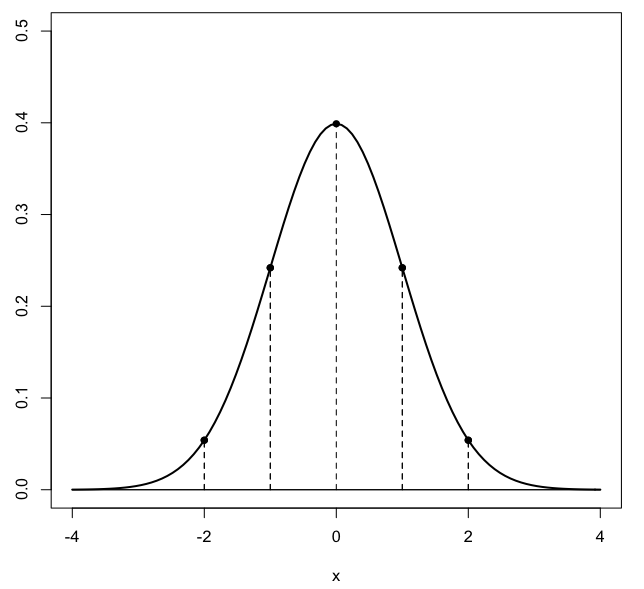
\includegraphics [scale=0.4] {gauss3.png} \end{center}

%break
\title{Riemann sums}
\date{}

\begin{document}
\maketitle
\Large

\subsection*{Riemann sums}

We introduced integration as simply the reverse of differentiation.  The fundamental theorem of calculus gives us a means of evaluating integrals between two bounds.  

Starting with Courant, however, calculus courses have sought a more formal approach.  The first (though not the only) method is to compute what are called Riemann sums for the the area bounded under a curve.

\begin{center} 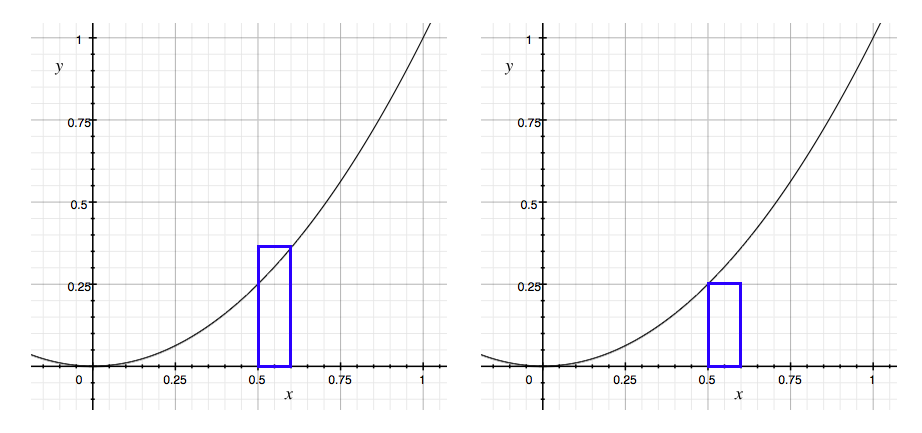
\includegraphics [scale=0.4] {riemann.png} \end{center}

Our first example is to calculate the area under the curve $f(x)=x^2$.  The areas of many small rectangles are added to form the sum. 

The key is to set up a calculation or expression for the area in terms of a variable number of rectangles, $N$.  Although any rectangle can only be an approximation to a curved surface, if we use many skinny rectangles the approximation will be very good, and \emph{in the limit} as $N \rightarrow \infty$, as we use an infinite number of rectangles, it will be exactly right.

The proof that it \emph{is} right is to show that the sum of a set of rectangles bounding the curve below, and the sum for a second set bounding the curve above, \emph{converge to the same limit} as $N \rightarrow \infty$.

Another way to see this is to look at this diagram from Newton's book \emph{De Analysi} (from Acheson's book \emph{The Calculus Story}).

 \begin{center} 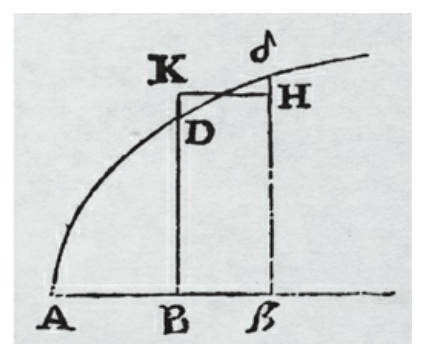
\includegraphics [scale=0.4] {newton_rect.png} \end{center}

Newton's argument is that if we draw a box as illustrated, there must be one height, one point along the top of the rectangle where the area under the curve but not in the box, to the right, is exactly equal to the area over the curve and in the box, to the left.  At that point, the errors exactly cancel.

If this point is always bounded by the $y$-values of the left and right sides of the box, then as the boxes get smaller and smaller, the balance point will always be included somewhere in the rectangle, so the answer will come out exactly right.  (This latter assumption breaks down at maxima and minima, but only for finite boxes.  Let's admire the diagram and move on to the actual method).

\subsection*{example}

We start with $x^2$.  It is the simplest power curve, and we actually know the answer due to work by Archimedes, called the \hyperref[sec:quad]{\textbf{quadrature}}.

Consider the region bounded by the $x$-axis, the $y$-axis, the line $x=1$, and the curve $y=x^2$.  

Partition the region on the $x$-axis between $x=0$ and $x=1$ into $N$ segments.  Each segment will contain a tall, thin rectangle that extends from the $x$-axis up to the curve.  

Here is a figure that illustrates the basic idea.  The region between $0$ and $1$ is divided into $10$ segments, so the width of each segment is $0.1$.  

In the left panel, the blue rectangle shown is the sixth segment;  its left and right bounds are $x = 0.5$ and $x = 0.6$.  The height is $x^2 = 0.6^2 = 0.36$.  The right panel is the same, except the height corresponds to the value at the left-hand bound $x^2 = 0.5^2$.
\begin{center} 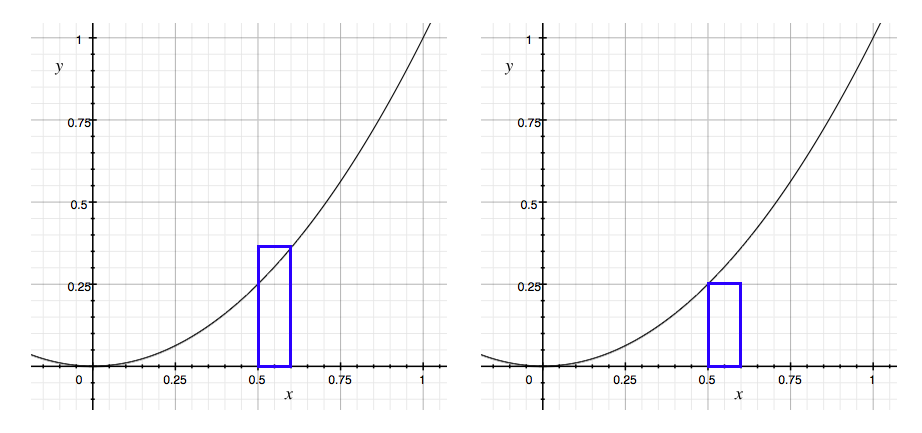
\includegraphics [scale=0.4] {riemann.png} \end{center}

We compute the area (using the first set of rectangles) as
\[  A = 0.1 (0.1^2 + 0.2^2 + \dots + 1.0^2) \]
\[  = 0.1 (0.01 + 0.04 + \dots + 1.0) \]
\[  = 0.1 (3.85) = 0.385 \]

This is obviously an over-estimate of the area (as it will be for any function that increases over the interval), but the trick is that as the number of rectangles becomes very large, the result will converge to the exact area we want.

\subsection*{area as a limit}
We divide the region into $N$ intervals.  Each interval has width $1/N$.  The $x$-values of the right hand side of these boxes are
\[ \frac{1}{N}, \frac{2}{N} \dots \frac{N}{N} \]

We can rewrite this as 
\[ \sum_{k=1}^N \frac{k}{N} \]

We will first compute the sums for the set of boxes that is an overestimate, it uses the $x$-value of the right hand side of each box times the width of each box:
\[ A = \sum_{k=1}^{N} f(\frac{k}{N}) \cdot \frac{1}{N}  \]

Since the function is $x^2$ this is
\[ A = \sum_{k=1}^{N} (\frac{k}{N})^2 \cdot \frac{1}{N}  \]

And since $N$ is a constant, it can be pulled out from the summation:
\[  A = \frac{1}{N^3} \sum_{k=1}^N k^2 \]

Now we need an expression for the sum of the squares of the first $N$ integers.  We will show below that the formula is $N \cdot (N+1)/2 \cdot (2N+1)/3$.  Distributing the factor of $1/N^3$ over each term, we obtain
\[ A = \frac{N}{N} \cdot \frac{N+1}{2N} \cdot \frac{2N+1}{3N} \]

If $N \rightarrow \infty$ and we take the limit, the result is the value of the integral
\[ I = \lim_{N \rightarrow \infty}  \frac{N}{N} \cdot \frac{N+1}{2N} \cdot \frac{2N+1}{3N} \]
\[ = 1 \cdot \frac{1}{2} \cdot \frac{2}{3} = \frac{1}{3}  \]

The reason is that as $N \rightarrow \infty$ the difference between $N$ and $N+1$ (or $N-1$ and $N$ becomes negligible compared to the size of $N$, therefore the ratio $(N+1)/2N$, for example is equal to $1/2$ in the limit.  In other words, for, say
\[ \lim_{N \rightarrow \infty}  \frac{1}{2N} \ (N + 1) = \lim_{N \rightarrow \infty} \frac{1}{2}(1 + \frac{1}{N}) = \frac{1}{2} \]

We must still compute the sums for the set of boxes that is an underestimate (for finite $N$), with the $x$-value used for the function taken from the left-hand side.  This is the series
\[ \frac{0}{N}, \frac{1}{N} \dots \frac{N-1}{N} \]

If the function is $f(x) = x^2$ the sum is
\[ A = \sum_{k=0}^{N-1} (\frac{k}{N})^2 \cdot \frac{1}{N}  \]

Since the first term is zero, just remove it and start the index from $1$
\[ A = \sum_{k=1}^{N-1} (\frac{k}{N})^2 \cdot \frac{1}{N}  \]

For the integral, we obtain
\[ I = \lim_{N \rightarrow \infty}  \frac{N-1}{N} \cdot \frac{N}{2N} \cdot \frac{2N-1}{3} \]
We obtain exactly the same result as before. This is really the proof that the method works.  In the limit of infinite $N$, the methods which over-estimate and under-estimate the area converge to the same value, therefore the result is exactly correct.

\subsection*{integer sums}

The first series that one usually sees of this type is 
\[ \sum_{k=1}^n k \]
The sum of the integers from $1 \rightarrow N$.  There is a simple formula
\[ \frac{n(n+1)}{2} \]

Here is a famous "proof without words":
\begin{center} 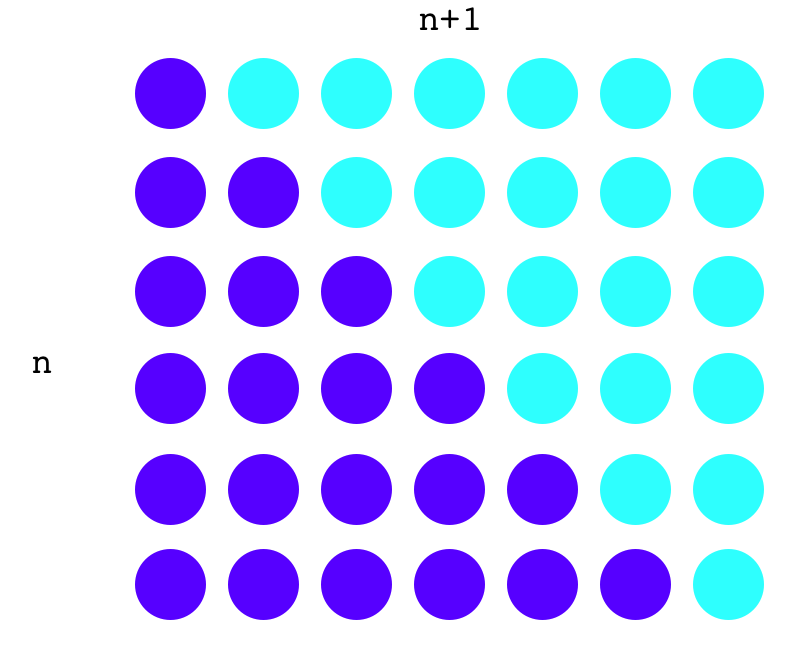
\includegraphics [scale=0.2] {sum_n.png}\end{center}

For Riemann sums, we need a series one level higher.  We need the sum of the squares of the first $n$ integers.  The answer is what we had before, multiplied by another term

\[ \frac{n(n+1)}{2} \ \frac{2n + 1}{3} \]

Here is another "proof without words."
\begin{center} 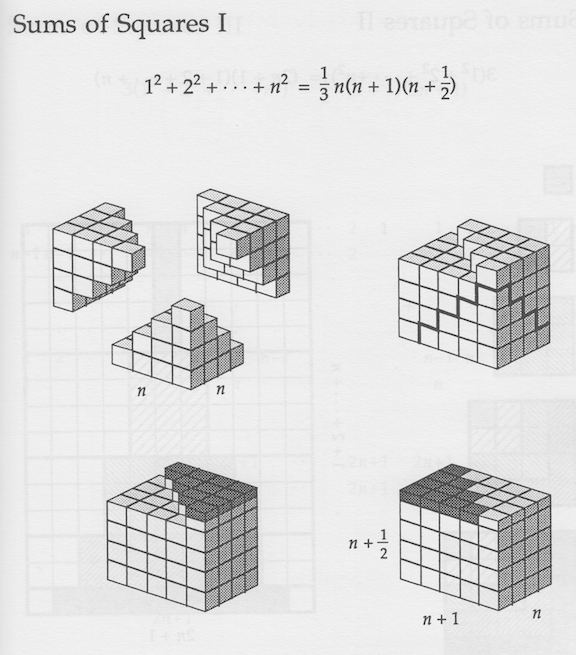
\includegraphics [scale=0.3] {sum_n2.png} \end{center}

For much more detail, see the chapter in the Addendum.

\subsection*{back to the Riemann sum}
We plug that expression into the Riemann Sum:
\[  = \frac{1}{N^3} \frac{N(N+1)}{2} \ \frac{2N + 1}{3} \]

Each of the terms in $N(N+1)(2N+1)$ is grouped with one of the $N$'s in the denominator at the left
\[  = \frac{1}{6} \ \frac{N}{N} \ \frac{(N+1)}{N} \ \frac{(2N + 1)}{N} \]

In the limit as $N$ gets very large.
\[  \lim_{N \rightarrow \infty}\frac{N}{N} = 1 \]
\[  \lim_{N \rightarrow \infty} \frac{N+1}{N} = \lim_{N \rightarrow \infty} 1 + \frac{1}{N} = 1 \]
\[  \lim_{N \rightarrow \infty} \frac{2N + 1}{N} = \lim_{N \rightarrow \infty} 2 + \frac{1}{N} = 2 \]

Thus, the final answer is $1/3$, which agrees with Archimedes.

\subsection*{n cubed}

The height of the first interval is $(1/N)^3$ and that of the $kth$ interval is $(k/N)^3$.  The total area is:
\[  \sum_{k=1}^N (\frac{k}{N})^3 \times \frac{1}{N}  \]

Since $N$ is a constant, it can be pulled out from the summation:
\[  \frac{1}{N^4} \sum_{k=1}^N k^3 \]

So now we need an expression for the sum of the cubes of the first $N$ integers.  

Yet another ingenious "proof without words."
\begin{center} 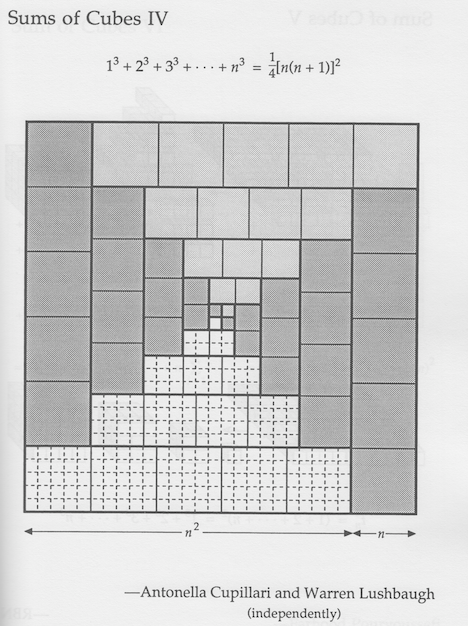
\includegraphics [scale=0.4] {sum_n3.png} \end{center}

\[   \sum_{k=1}^N k^3 = \frac{1}{4} \ [ \ n (n+1) \ ] ^2  \]
\[ = \frac{1}{4} \ N (N+1) N (N+1) \]

As before, each of the four factors of $N$ in the denominator cancels an $N$ or $N+1$ on top and we're left with just $1/4$.

It turns out that if you let the interval be $[0,b]$ or even $[a,b]$, we obtain the expressions you will be used to from integral calculus, namely
\[ \int_a^b n^2 = \frac{n^3}{3} \ \bigg |_a^b \]
and
\[ \int_a^b n^3 = \frac{n^4}{4} \ \bigg |_a^b \]


\end{document}